%----------------------------------------------------------------------------------------
%	PACKAGES AND OTHER DOCUMENT CONFIGURATIONS
%----------------------------------------------------------------------------------------
\documentclass[12pt]{article}
\usepackage[protrusion=true,expansion=true]{microtype} % Better typography
\usepackage{graphicx} % Required for including pictures
\usepackage{wrapfig} % Allows in-line images
\usepackage[utf8]{inputenc}
\usepackage{mathpazo} % Use the Palatino font
\usepackage[T1]{fontenc} % Required for accented characters
\usepackage{verbatim} % comentarios
\linespread{1.05} % Change line spacing here, Palatino benefits from a slight increase by default

\makeatletter
\renewcommand\@biblabel[1]{\textbf{#1.}} % Change the square brackets for each bibliography item from '[1]' to '1.'
\renewcommand{\@listI}{\itemsep=0pt} % Reduce the space between items in the itemize and enumerate environments and the bibliography

\renewcommand{\maketitle}{ % Customize the title - do not edit title and author name here, see the TITLE block below
\begin{flushright} % Right align
{\LARGE\@title} % Increase the font size of the title

\vspace{50pt} % Some vertical space between the title and author name

{\large\@author} % Author name
\\\@date % Date

\vspace{40pt} % Some vertical space between the author block and abstract
\end{flushright}
}


\begin{document}

\begin{titlepage}

\newcommand{\HRule}{\rule{\linewidth}{0.5mm}} % Defines a new command for the horizontal lines, change thickness here

\begin{center}
 
%----------------------------------------------------------------------------------------
%	HEADING SECTIONS
%----------------------------------------------------------------------------------------

\textsc{\LARGE Benemerita Universidad Autonoma de Puebla}\\[1.2cm] % Name of your university/college
\textsc{\Large PROYECTO FINAL}\\[0.8cm] % Major heading such as course name
\textsc{\Large Sistemas Operativos II}\\[0.5cm] % Major heading such as course name
\textsc \emph{\large Profesor: Luis Enrique Colmenares Guillen}\\[0.3cm] % Minor heading such as course title

%----------------------------------------------------------------------------------------
%	TITLE SECTION
%----------------------------------------------------------------------------------------

\HRule \\[0.4cm]
{ \huge \bfseries Multiplicacion de matrices}\\[0.4cm] % Title of your document
\HRule \\[1cm]
%----------------------------------------------------------------------------------------
%	AUTHOR SECTION
%----------------------------------------------------------------------------------------
\textsc{\Large Autores}\\[0.3cm] % Major heading such as course name
\begin{minipage}{0.5\textwidth}
\begin{flushleft} \large
\centering \textsc{Placido Velazco Cesar Eduardo\\   201214687} % Your name
\end{flushleft}
\end{minipage}
~
\begin{minipage}{0.3\textwidth}
\begin{flushright} \large
\centering \textsc{Vazquez Martinez Josue\\201245534} % Supervisor's Name
\end{flushright}
\end{minipage}\\ [1cm]

{\large Noviembre 29, 2017}\\[1cm]

%----------------------------------------------------------------------------------------
%	LOGO SECTION
%----------------------------------------------------------------------------------------


\includegraphics[width=5cm,height=5cm,keepaspectratio]{buap.png} % Include a department/university logo - this will require the graphicx package
 
%----------------------------------------------------------------------------------------
\end{center}

\title{\textbf{PROGRAMACIÓN CON MPI}\\ % Title
Multiplicacion de matrices} % Subtitle

\author{\textsc{Proyecto final} % Author
\\{\textit{Benemerita Universidad Autonoma de Puebla}}} % Institution

\date{\today} % Date

%----------------------------------------------------------------------------------------


\maketitle % Print the title section

%----------------------------------------------------------------------------------------
%	ABSTRACT AND KEYWORDS
%----------------------------------------------------------------------------------------

%\renewcommand{\abstractname}{Summary} % Uncomment to change the name of the abstract to something else

\begin{abstract}
Actualmente existen problemas que demandan mucho tiempo de procesamiento en una
computadora, por ejemplo: predicción del estado del tiempo, algoritmos para trazar rutas de aviones, simulación de fenómenos naturales, peticiones a una base de datos, análisis de información, conversión de formatos (de video principalmente), etc. Algunos de ellos, además de utilizar tiempo en CPU necesitan gran cantidad de memoria. Solucionar estos problemas puede tardar desde minutos hasta días o meses.
Desde sus inicios, la solución para resolver estos problemas fue fabricar computadoras con procesadores cada vez más rápidos, pero con el paso de los años, se alcanzaron límites físicos que impedían continuar con esta tendencia. Entonces se desarrollaron máquinas con varias unidades de procesamiento.
Actualmente, todas (o casi todas) las computadoras tienen por lo menos procesadores con dos núcleos y pueden ser adquiridas a precios accesibles. Incluso es raro encontrar dispositivos móviles (como celulares y tablets) que tengan un solo CPU.
A pesar de esto, las soluciones a muchos problemas de cómputo se realizan de manera secuencial,desperdiciando recursos hardware, esto debido a que aún es poca la cultura de desarrollo de aplicaciones que aprovechen las capacidades del procesamiento paralelo. Sin embargo, en la actualidad, existen diferentes herramientas para el desarrollo de programas paralelos que hace que esta actividad se vuelva más sencilla, atractiva y factible, obteniendo software que reduce eltiempo de ejecución considerablemente, así como soluciones de manera más rápida.
Por lo anterior, el objetivo de este trabajo utilizar una bilioteca estándar para programación paralela bajo el paradigma de comunicación de procesos mediante pasaje de mensajes (MPI).
El ejercicio propuesto por el DR. Luis Enrique Colmenarse Guillen es un escenario	multiprocesamiento que consiste	en realizar la multiplicación de Matrices nxn en los siguientes tamaños 16, 32, 64, 128, 256, 512, 1024, 2048;
Se	llenaran	los	valores	de	las	matrices	con	valores	densos	y	pseudoaleatorios	de	
números	entre	1000	y	2000, Se	utilizaran	enteros	y	flotantes, Se	repetirán	100	veces	la	multiplicación	para	encontrar	un	promedio,Se	graficará	tiempo	total	y	memoria total, estas graficas seran 	con	Gnuplot 
\end{abstract}


\hspace*{3,6mm}\textit{Keywords:} OpenMPI ,Paralelo ,Multiplicacion% Keywords

\vspace{30pt} % Some vertical space between the abstract and first section

%----------------------------------------------------------------------------------------
%	ESSAY BODY
%----------------------------------------------------------------------------------------

\section*{MPI}
Es una interfaz de paso de mensajes altamente eficiente y portable para satisfacer las necesidades actuales en la computación de alto rendimiento a través de la definición de un estándar de paso de mensajes universal.\\
Es un estándar de programación en paralelo creado en 1993. Es abierto por fabricantes y usuarios.Principalmente, incluye interfaces para FORTRAN, C y C++.
La unidad básica son los procesos.\\ 
Un proceso es una entidad formada por los siguientes dos elementos principales:\\
1. Imagen binaria del programa, cargada parcial o totalmente en memoria física. La imagen
binaria está formada por las instrucciones y datos del programa.\\
2. Área de memoria para almacenar datos temporales, también conocida como pila.\\
 \\
El funcionamiento, a grandes rasgos, es:\\
1.- A cada proceso se le asigna un identificador interno.\\
2.- Tienen espacios de memoria independientes.\\
3.- Intercambio de información por paso de mensajes.\\
4.- Para realizar la comunicación, introduce el concepto de comunicadores, que agrupa a los procesos implicados en una ejecución paralela. Estos procesos pueden intercambiarse
mensajes.\\

%------------------------------------------------
\section*{Algoritomo Secuencial}
La implementacion secuencial de una multiplicacion de matrices conciste en una iteracion triple para poder operar con todos los elementos de las matrices.
Podremos observar mejor en la siguiente figura.
\begin{figure}[htb]
\centering
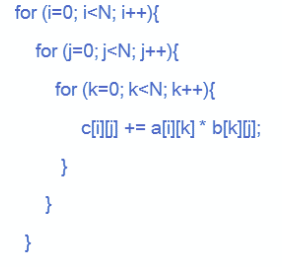
\includegraphics[width=0.7\textwidth]{secuencial.png}
\caption{Iteraciones del algoritmo secuencial. }
\end{figure}\\
De este modo se pude observar que el algoritmo funciona bien pero con matrices muy grandes el algoritmo es muy poco eficiente respecto al tiempo.

\section*{Algoritomo de Cannon}
Utiliza una malla con conexiones entre los elementos de cada lado para desplazar los elementos de A hacia la izquierda y los de B hacia arriba.\\
El algoritmo sigue los siguientes pasos:\\
	1. El procesador Pij tiene los elementos aij y bij\\
	2. La fila i-ésima de A se desplaza i posiciones a la izquierda, y la columna j-		ésima de B se desplaza j posiciones hacia arriba, y todo esto teniendo en cuenta 		que el elemento que sale por un extremo entra por el otro. Con este paso se 			consigue que el procesador Pij contenga los elementos aij+i y bi+jj, que son 			necesarios para calcular cij.\\
	3. Cada procesador multiplica su par de elementos.\\
	4. Cada fila de A se desplaza una posición a la izquierda, y cada columna de B una posición hacia arriba.\\
	5. Cada procesador multiplica su nuevo par de elementos, y suma el resultado al anterior.\\
	6. Se repiten los pasos 4 y 5 hasta terminar, es decir n-1 desplazanientos.\\
	Como podemos aprecian en figure 1.

\begin{figure}[htb]
\centering
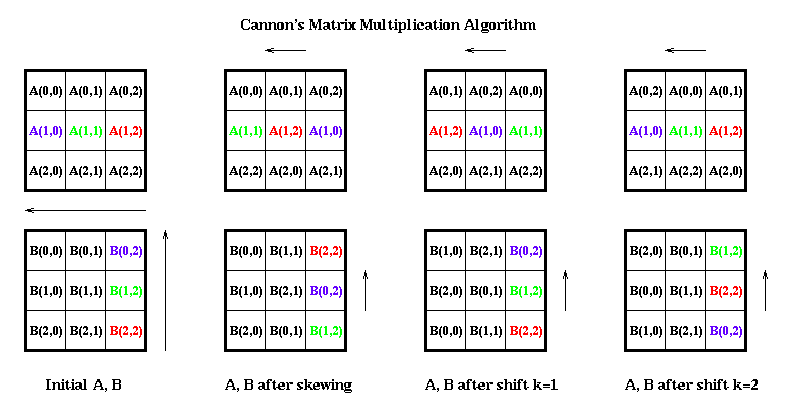
\includegraphics[width=0.7\textwidth]{c.png}
\caption{Algoritmo Cannon }
\end{figure}


\section{Instalación}
Este proyecto se realizo en un entorno Linux usando la distribución Ubuntu 16.04 como se especifico en el reporte, tambien se especifica el hardware utilizado el cual, en caso de que se quiera implementar en otro equipo, tendria que ponerse especial atencion en si cumplen o no o las formas de adaptarlo.\\

Libreria MPI\\
Ya que estamos en nuestro sistema operativo deberemos tener instalada la liberia MPI, la version 1.0 emostro tener problemas para ejecutar algunas funciones, sin embargo, la version que no presentó ningun problema fue la 3.0.0 la cual usaremos durante toda este manual. Para verificar que version de MPI se está ejecutando utilice el comando mpirun -version. Esta version puede ser encontrada en la pagina: https://www.open-mpi.org/software/ompi/v3.0/ Basta con compilar la libreria y listo.\\

Libreria GNUPLOT\\
Una vez que tenemos lista la libreria deberemos descargar tambien las librerias  gnuplot para poder visualizar correctamente las graficas generadas por el programa, puede encontrar los archivos de descarga e informacion en la pagina: http://gnuplot.sourceforge.net/\\

Compilacion\\
Para poder generar el archivo .out tendremos que utilizar el siguiente comando:
mpicc MatrixIntCannonPlot.c -o MatrixIntCannonPlot -lm.\\
La primera instruccion -mpicc- es para compilar nuestro archivo, que en este caso se llama MatrixIntCannonPlot.c, por ello el nombre va como el segundo argumento, recuerde agregar la extencion del programa ".c", despues le especificamos al compilador el nombre del archivo .out que queremos que nos genere, este paso es opcional, sin embargo, es aconsejable agregarlo para evitar confucion mas adelante en cuanto que .out pertenece a que .c, la ultima instruccion es -lm la cual hace un llamado a la libreria math.h la cual de no agregarse, manda un error de que no se encuentra dicha libreria, a pesar de que la tenemos declarada en la cabecera de nuestro programa, basta con agregar el comando -lm para que esto desaparesca.\\ 

Ejecucion.\\
Antes de explicar el comando usado para ejecutar el programa previamente compilado, debemos entender algo, MIP no permite la "sobre subscripcion", al menos no por default, lo cual significa que si tenemos 4 nucleos fisicos y otros 4 logicos MPI nos limitará a 4, aun que le especifiquemos que deseamos usar mas,por ello, usaremos el comando: mpirun --map-by socket:OVERSUBSCRIBE -np 8 MatrixIntCannonPlot, el primer comando -mpirun- es el comando que se encarga de ejecutar los archivos compilados, --map-by socket:OVERSUBSCRIBE se encarga de "desbloquear" los demas nucleos para que podamos usarlos con toda libertad, -np  es donde se debe de especificar el numero de nucleos que queremos usar, ya sea 1, 2, 4 u 8, esto dependerá de la arquitectura disponible y de el ejemplo que nos gustaria ver. Cabe destacar que el numero de nucleos tales como 3, 5 y 6 no fueron agregados, esto no quiere decir que no sea posible ejecutar ese numero de nucleos, simplemente que en nuestros ejemplos, los cuales son matrices cuadradas de 16, 32 ,64, 128, 256, 512, 1024 y 2048 no son divisibles entre esos numeros de nucleos, y recordemos que lo que realiza MPI es dividir la matriz entre el numero de procesadores asignados. \\

Resultados.\\
Lo que veremos a continuacion es una serie de resultados, dependiendo de el numeor de nucleos que ejecutamos será la cantidad de respuestas que obtendremos, por ejemplo, si en la ejecucion usamos -np 1 veremos un mensaje en la consola parecido a Promedio: 0.002321 y una grafica donde se muestra los tiempos y el uso de memoria, y dependiendo de el numero de nucleos que hayamos usado sera el numero de promedios que veremos.




%------------------------------------------------

\section*{Conclusion}
%\begin{comment}



%----------------------------------------------------------------------------------------
%	BIBLIOGRAPHY
La multiplicacion de matrices es usualmente un proceso que requiere muchos recursos para ser ejecutada, con un algoritmo secuencial los tiempos crecen exponencialmente a medida de que crece el tamaño de la matriz, MPI es una libreria que nos ayuda paralelizando nuestros procesos, haciendo que la tarea sea dividida entre cierto numero de procesadores, sin embargo, esto no nos garantiza que el tiempo de procesamiento se vea reducido a la mitad si pasamos de 1 a 2 nucleos, muchas veces el tiempo de ejecucion siguie siendo bastante extenso, al usar un algoritmo paralelo como es Cannon acortams aun mas el tiempo que tarda en encontrar una solucion, la diferencia es enorme, pues estamos multiplicando matrices con valores aleatorios de entre 1000 y 2000 y estamos repitiendo el proceso 100 veces, aun asi el proceso, como ya lo vimos en las tablas, no tarda mucho. El problema con Cannon es que a medida que aumenta el tañano de la matriz, la eficiencia del algoritmo cae, haciendo el procesamiento cada vez mas lento, sin importar que aumentemos el numero de nucleos, quedando demostrado que Cannon es eficiente en matrices pequeñas, quiza si se necesitan dimensiones mayores sea necesario implementar otro algoritomo como Fox, Indexado, etc.
%----------------------------------------------------------------------------------------

%\bibliographystyle{unsrt}
%\end{comment}

\section*{Bibliografia}
\begin{comment}



%----------------------------------------------------------------------------------------
%	BIBLIOGRAPHY
%----------------------------------------------------------------------------------------

\bibliographystyle{unsrt}
\end{comment}


\bibliography{sample}


Libreria MPI para Linux\\
https://www.open-mpi.org/software/ompi/v3.0/\\

Libreria GNUPLOT\\
http://gnuplot.sourceforge.net/\\

Notas de Over:SUBSCRIBE\\
https://www.open-mpi.org/faq/?category=runningslots-without-hostfiles\\

Caracteristicas del procesador\\
https://ark.intel.com/products/75117/Intel-Core-i7-4700MQ-Processor-6M-Cache-up-to-3-40-GHz\\






\end{titlepage}
\end{document}